\documentclass{ctexart}
\usepackage{EC}
\begin{document}
\section{硫及其化合物}
\subsection{单质硫}
\subsubsection{\ce{S8}:$\alpha$-正交硫,$\beta$-单斜硫和$\gamma$-单斜硫}
\begin{substance}[正交$\mbf{\alpha}$-\ce{S8}]
    硫最常见的,也是热力学上最稳定的单质为正交$\mbf{\alpha}$-\ce{S8}(简称正交硫).这是一种黄色固体,具有优良的绝缘性和绝热性.
\end{substance}
正交硫中含有$D_{4\text d}$点群的\ce{S8}分子,其结构颇像皇冠.
\begin{figure}[H]
    \centering
    \subfigure[\ce{S8}分子的俯视图]{
        \begin{minipage}[b]{.45\linewidth}
            \centering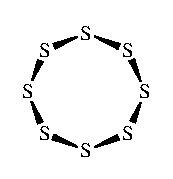
\includegraphics{picture/S8-1.eps}
        \end{minipage}
    }
    \subfigure[\ce{S8}分子的侧视图]{
        \begin{minipage}[b]{.45\linewidth}
            \centering
\includegraphics{picture/S8-2.eps}
        \end{minipage}
    }
    \caption{\ce{S8}分子的立体结构}
\end{figure}
加热$\alpha$-\ce{S8}至$95.3\tccentigrade$可使其转变为$\beta$-单斜\ce{S8}.将硫熔融后缓慢冷却可以得到$\gamma$-单斜\ce{S8}.这两种晶型中都由\ce{S8}分子组成,区别只在于排列方式不同.
\subsubsection{\ce{S6}:$\ep$-硫}
$\ep$-硫由\ce{S6}分子构成,其颜色为橙红色,分子构象与环己烷的椅式六元环一致.这种同素异形体可以由下面的反应制得:
\begin{center}
    \ce{H2S4 + S2Cl2 ->T[\ce{Et2O}] S6 + 2HCl}
\end{center}
\subsubsection{\ce{S}的小分子:\ce{S2}与\ce{S3}}
低压高温的硫蒸汽中存在\ce{S2}与\ce{S3}分子.\ce{S3}分子呈现樱桃红色,结构与\ce{O3}类似.\ce{S2}分子呈现紫色,结构与\ce{O2}类似.
\subsection{$\mbf{-2}$氧化态}
\subsubsection{\ce{H2S}}
我们照例从氢化物开始.
\begin{substance}[\ce{H2S}]
    硫化氢,化学式为\ce{H2S},是无色的具有恶臭的剧毒气体.\ce{H2S}在空气中燃烧时发出浅蓝色的火焰.\ce{H2S}易溶于水,室温下在纯水中的溶解度大约为$1\text{ mol}\cdot\text{L}^{-1}$.
\end{substance}
\ce{H2S}是较弱的酸,并且是一种中等强度的还原剂.将\ce{H2S}溶液置于空气中,溶液将缓慢地变浑浊,其中生成了\ce{S}单质沉淀.
\subsubsection{金属元素的硫化物}
自然界有许多重要矿物以及金属元素的矿石是硫化物,这些矿石最重要的用途是自其中冶炼出金属.这些矿物中比较重要的列举如下:
\begin{table}[H]\centering
        \begin{tabular}{|c|c|c|c|c|c|}
        \hline
        名称 & 理想化学式 & 名称 & 理想化学式 & 名称 & 理想化学式 \\\hline
        辉钼矿 & \ce{MoS2} & 方铅矿 & \ce{PbS} & 雄黄 & \ce{As4S4} \\\hline
        雌黄 & \ce{As2S3} & 黄铁矿 & \ce{FeS2} & 白铁矿 & \ce{FeS2} \\\hline
        辉锑矿 & \ce{Sb2S3} & 黄铜矿 & \ce{CuFeS2} & 砷黄铁矿 & \ce{FeAsS} \\\hline
        辉铜矿 & \ce{Cu2S} & 闪锌矿 & \ce{ZnS} & 朱砂 & \ce{HgS} \\\hline
        \end{tabular}
\end{table}
所有硫化物矿中以黄铁矿丰度最大,这也是硫单质的主要来源.这些硫化物的性质将在对应元素的章节提及.
\subsection{多硫阴离子}
多硫阴离子\ce{S_n^2-}$\left(n=2,3,4,5\right)$可以由\ce{S^2-}与\ce{S}单质反应得到.这些离子为黄色,并且颜色随着$n$的增加而加深.\\
\indent 有关多硫离子,值得提到的一点是石硫合剂.它是\ce{Ca(OH)2}与\ce{S}单质反应得到的,通常以红黄色水溶液的形式用作病虫害防治.\\
\indent 另一个有趣的配合物,也是无机化合物中鲜有的具有手性的例子,是\ce{Pt^{\ce{IV}}}与\ce{S5^2-}的配离子.它的结构如下所示.
\begin{figure}[H]
    \centering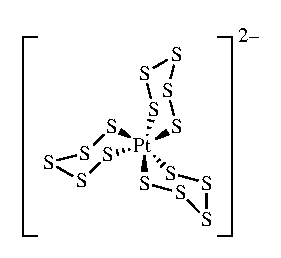
\includegraphics{picture/PtS15.eps}
    \caption{\ce{PtS15^2-}的结构}
\end{figure}
\subsection{$\mbf{+4}$氧化态}
\subsubsection{\ce{SO2}}
\ce{SO2}是硫的常见氧化物.
\begin{substance}[\ce{SO2}]
    二氧化硫,化学式为\ce{SO2},是无色,有窒息性臭味的有毒气体.\ce{SO2}的熔点为$-75.5\tccentigrade$,沸点为$-10.0\tccentigrade$.\ce{SO2}气体易溶于水.
\end{substance}
工业上大规模制备\ce{SO2}是由硫或\ce{H2S}在空气中燃烧,或锻烧黄铁矿.\ce{SO2}也是一种常见的大气污染物.工业上生产的\ce{SO2}主要用来制备硫酸其他如漂白,杀菌,食物保存,冷冻或作为非水溶剂等.
\subsubsection{亚硫酸及其盐}
亚硫酸仅存在于低浓度的\ce{SO2}水溶液中,难以作为纯物质被单独分离.亚硫酸盐则稳定得多,各种阳离子都能与它们形成稳定的盐.\\
\indent 亚硫酸氢根\ce{HSO3-}有两种互变异构体.占主要的那种是具有$C_{3\text v}$对称性的\ce{HSO3-}而非\ce{HOSO2^-}.
\begin{figure}[H]
    \centering\includegraphics{picture/HSO3-.eps}
    \caption{\ce{HSO3-}的两种互变异构体的结构}
\end{figure}
\indent \ce{HSO3-}和\ce{SO3^2-}为中等强度的还原剂.它们与\ce{I2}能发生定量的反应:
\begin{center}
    \ce{HSO3- + I2 + H2O <=> HSO4- + 2H+ + 2I-}
\end{center}
在强还原剂的存在下,它也能被还原:
\begin{center}
    \ce{2SO3^2- + 2H2O + 2Na(Hg) -> S2O4^2- + 4OH- + 2Na+}\\
    \ce{2SO3^2- + 4HCOO- -> 2S2O3^2- + 2C2O4^2- + 2OH^- + H2O}
\end{center}
\subsubsection{\ce{H2S2O5}}
与\ce{H2SO3}一样,\ce{H2S2O5}也没有得到纯的化合物.\ce{S2O5^2-}的盐可以容易地由亚硫酸氢盐浓缩制得:
\begin{center}
    \ce{2HSO3^- <=> S2O5^2- + H2O}
\end{center}
与\ce{HSO3-}一样,\ce{S2O5^2-}的结构也不同寻常,其中的两个\ce{S}并不等价,而是由一根\ce{S-S}键相连.
\begin{figure}[H]
    \centering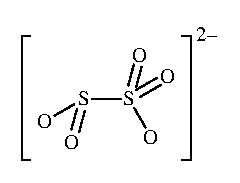
\includegraphics{picture/S2O52-.eps}
    \caption{\ce{S2O5^2-}的结构}
\end{figure}
\subsection{$\mbf{+6}$氧化态}
\subsubsection{\ce{SO3}}
\ce{SO3}也是硫的常见氧化物.
\begin{substance}[\ce{SO3}]
    三氧化硫,化学式为\ce{SO3},是无色针状固体或液体,有刺激性气味.\ce{SO3}的熔点为$16.9\tccentigrade$,沸点为$45\tccentigrade$,极易溶于水.
\end{substance}
气态的\ce{SO3}为平面型分子.液态的\ce{SO3}主要为其三聚体\ce{S3O9},其结构如下.
\begin{figure}[H]
    \centering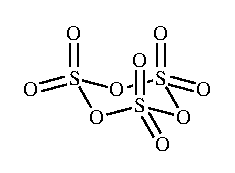
\includegraphics{picture/S3O9.eps}
    \caption{\ce{SO3}的三聚体的结构}
\end{figure}
固态\ce{SO3}有两种晶型,一种是由\ce{S3O9}构成的$\gamma$-\ce{SO3};当微量水存在时,可以结晶为针状的$\beta$-\ce{SO3},其中含有长链聚合物\ce{HO(SO3)_nH}.另一种更稳定的晶型$\alpha$-\ce{SO3}中有复杂的交联结构\footnote{同一温度下这三种晶型的蒸气压大小顺序为$\alpha<\beta<\gamma$,因此加热$\alpha$-\ce{SO3}至熔化时会导致其蒸气压突然升高,巨大的压力可以冲破加热它的玻璃管.这一现象称为$\alpha$爆炸.}.\\
\indent 工业上制备\ce{SO3}通常在催化剂(例如$\ce{V2O5}$)的存在下氧化\ce{SO2}得到;随后一般被通入$98.3\%$硫酸中吸收,这就是工业制硫酸的方法.
\subsubsection{\ce{SO4}}
这种化合物中含有过氧键,实际上可以写作\ce{SO2(O2)}.
\subsubsection{\ce{H2SO4}}
硫酸是一种重要的物质.
\begin{substance}[\ce{H2SO4}]
    硫酸,化学式为\ce{H2SO4}.无水硫酸为无色粘稠的液体,与水以任意比例混溶,混合过程放出大量的热.
\end{substance}
在无水硫酸中存在一系列平衡:
\begin{center}
    \ce{2H2SO4 <=> H3SO4+ + HSO4-}\\
    \ce{2H2SO4 <=> H3O+ + HS2O7-}\\
    \ce{H3O+ + HSO4- <=> H2SO4 + H2O}\\
    \ce{HS2O7- + H3SO4+ <=> H2S2O7 + H2SO4}\\
    \ce{H2S2O7 <=> H2SO4 + SO3}
\end{center}
因此,无水硫酸中事实上至少含有七种组分.这也经常被用于考察平衡计算.无水硫酸的许多性质也是由这些物种造成的.\\
\indent 大多数物质在无水\ce{H2SO4}中都作为碱存在.少数物质,例如\ce{H2S2O7},\ce{HSO3F}等可以作为酸将\ce{H2SO4}质子化.另一个特殊的例子是硼酸溶于无水硫酸形成的四硫酸氢硼酸:
\begin{center}
    \ce{H3BO3 + 3H2S2O7 -> H3SO4+ + [B(HSO4)4]- + H2SO4}
\end{center}
\indent 需要说明的是,如果某一反应在浓硫酸体系生成\ce{H2O},那么最好将其写作\ce{H3OHSO4}或\ce{H2O.nH2SO4}的形式.\\
\indent 稀硫酸的性质,主要是\ce{SO4^2-}和\ce{H^+}的性质.这部分内容已经在高中化学中学过,这里就不作介绍了.
\subsubsection{\ce{H2SO5}与\ce{H2S2O8}}
无水过一硫酸\ce{H2SO5}(亦被称作Caro酸)可由无水过氧化氢和氯磺酸反应值得,然而此物质少有用处,主要作为电解法制备\ce{H2S2O8}及其盐的副产物而出现.\\
\indent 过二硫酸\ce{H2S2O8}为无色固体,可以以任意比例混溶于水中;熔点为$65\tccentigrade$,熔化时分解.\ce{(NH4)2S2O8}和\ce{K2S2O8}是过二硫酸的两种最重要的盐,它们都易溶于水(但\ce{K2S2O8}溶解得十分缓慢).这些盐比酸更容易制备,它们都已实现工业化生产,其法是由相应的硫酸盐进行阳极氧化.\\
\indent 过二硫酸及其盐常被用作强氧化剂.除去少数物质,例如\ce{F2},\ce{H2N2O2},\ce{O}和\ce{OH}等,电对$\ce{S2O8^2-}/\ce{HSO4-}$的电极电势比其它水溶液中的电对都要高.
\subsection{硫代硫酸及其盐}
游离的硫代硫酸遇水即发生迅速而复杂的分解\footnote{这也是碘量法需要控制溶液pH在近中性的原因}.一种典型的分解方式为
\begin{center}
    \ce{H2S2O3 -> H2S + SO2}
\end{center}
硫代硫酸盐则相对稳定得多,可以由\ce{HS^-}与\ce{HSO3^-}反应制得:
\begin{center}
    \ce{2HS- + 4HSO3- -> 2S2O3^2- + 3H2O}
\end{center}
也可以由\ce{SO3^2-}与硫单质的反应制得:
\begin{center}
    \ce{8Na2SO3 + S8 -> 8Na2S2O3}
\end{center}
\indent \ce{S2O3^2-}的结构与\ce{SO4^2-}极为相似,只是把其中一个端基\ce{O}替换为\ce{S}即可.
\begin{substance}[\ce{Na2S2O3.5H2O}]
    海波/大苏打,即五水合硫代硫酸钠,化学式为\ce{Na2S2O3.5H2O},是一种无色晶体,熔点$48.5\tccentigrade$,易溶于水.
\end{substance}
海波在照相业\footnote{尽管这一行业现在已经很少用这种古老的办法摄影了.}中用作定影剂,用于溶解未反应的\ce{AgBr},反应的方程式为
\begin{center}
    \ce{AgBr + 3S2O3^2- -> [Ag(S2O3)3]^5- + Br-}
\end{center}
此外,硫代硫酸钠是一种中等强度的还原剂.\ce{S2O3^2-}与\ce{I2}定量地发生反应,这是碘量法的理论基础:
\begin{center}
    \ce{2S2O3^2- + I2 -> S4O6^2- + 2I-}
\end{center}
更强的氧化剂可以将其直接氧化为\ce{S^{VI}}:
\begin{center}
    \ce{S2O3^2- + 4Cl2 + 5H2O -> 2HSO4- + 8H+ + 8Cl-}
\end{center}
\ce{Br2}的氧化性介于\ce{I2}和\ce{Cl2}之间,根据不同条
件,\ce{S2O3^2-}可作为单电子或八电子还原剂.用也\ce{S2O3^2-}和\ce{Br2}的浓溶液进行滴定,然后将两种溶液各稀释100倍再进行滴定,将发现\ce{S2O3^2-}的滴定度正好增加为8倍.
\subsection{连硫酸及其盐}
\subsubsection{连二硫酸及其盐}
连二硫酸盐通常可由亚硫酸盐进行氧化制得.工业上由水合\ce{MnO2}或\ce{Fe2O3}的悬浊液对\ce{SO2}的水荣溶液进行氧化即得相应的连二硫酸盐:
\begin{center}
    \ce{2MnO2 + 3SO2 ->T[aq,$0\tccentigrade$] MnSO4 + MnS2O6}\\
    \ce{Fe2O3 + 3SO2 ->T[aq,$0\tccentigrade$] FeSO3 + FeS2O6}
\end{center}
通过复分解反应即可制备其它连二硫酸盐.
\subsubsection{连多硫酸\ce{H2S_nO6}}
连多硫酸及其盐具有悠久历史和系统的化学研究工作.1808年John Dalton将\ce{H2S}与\ce{SO2}水溶液作用的研究,其中含有各种连硫酸.1846年,H.W.F.Wackenroder对这类溶液又进行了系统的研究,因此该体系以他的名字命名.除了这种方法之外,各种连多硫酸盐还可以通过以下方法制备:
\begin{center}
    \ce{2Na2S203 + 4H2O2 -> Na2S3O6 + Na2SO4 + 4H2O}\\
    \ce{2Na2S203 + I2 -> Na2S4O6 + 2NaI}
\end{center}
连五硫酸和连六硫酸盐的制备过程较复杂,这里就不再介绍了.
\subsection{连二亚硫酸及其盐}
连二亚硫酸的无水盐是稳定的,但在酸性条件下将发生分解:
\begin{center}
    \ce{2S2O4^2- + H2O -> S2O3^2- + 2HSO3^-}
\end{center}
强碱性条件下亦将发生分解:
\begin{center}
    \ce{2S2O4^2- + 6OH^- -> 5SO3^2- + S^2- + 3H2O}
\end{center}
连二亚硫酸盐加热时也将发生分解,分解方式和酸性条件下的歧化类似:
\begin{center}
    \ce{2Na2S2O4 ->T[$\Delta$] Na2S2O3 + Na2SO3 + SO2}
\end{center}
\indent \ce{S2O4^2-}具有明显的重叠式结构,并且\ce{S-S}键明显偏长.事实上,\ce{S2O4^2-}的水溶液中也有少量\ce{SO2^.-}存在.\\
\indent 用\ce{Zn}粉等还原剂或电解还原\ce{SO3^2-}即可制得\ce{S2O4^2-}.连二亚硫酸盐在工业上广泛用作还原剂;它还可以还原各种重金属离子.这类反应较多地被用于净化污水.
\subsection{硫的卤化物与卤氧化物}
\subsubsection{硫的氟化物} 硫的氟化物的性质和其它卤素的卤化物有一定程度的区别,因此分开讨论.
\begin{enumerate}[label=\tbf{\arabic*},topsep=0pt,parsep=0pt,itemsep=0pt,partopsep=0pt]
    \item \tbf{\ce{S2F2}}\\
        硫和\ce{AgF}在干燥的容器中氟化可以得到\ce{FSSF}.在有碱金属氟化物存在时,这种物质容易异构化形成\ce{SSF2}.这是一个简单的键合异构的例子.当然,\ce{SSF2}本身也可以由\ce{SO2}溶剂中的\ce{KF}与\ce{S2Cl2}反应得到:
        \begin{center}
            \ce{2KSO2F + S2Cl2 ->T[\ce{SO2}] SSF2 + 2KCl + 2SO2}
        \end{center}
        两者的结构示意如下.
        \begin{figure}[H]
            \centering
            \subfigure[\ce{FSSF}的结构]{
                \begin{minipage}[b]{.45\linewidth}
                    \centering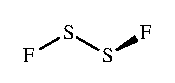
\includegraphics{picture/S2F2.eps}
                \end{minipage}
            }\subfigure[\ce{SSF2}的结构]{
                \begin{minipage}[b]{.45\linewidth}
                    \centering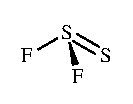
\includegraphics{picture/SSF2.eps}
                \end{minipage}
            }
            \caption{两种\ce{S2F2}的结构}
        \end{figure}
    \item \tbf{\ce{SF2}}\\
        \indent \ce{SF2}的稳定性并不如与它相似的\ce{H2S}或\ce{SCl2},因而难以得到.这种化合物需要\ce{KF}对\ce{SCl2}氟化后的一系列硫的氟化物中分离制得.
    \item \tbf{\ce{SF4}}\\
        \indent 相比前面几种物质,\ce{SF4}是一种稳定得多的氟化物.\ce{SF4}最好由下面的方法制备:
        \begin{center}
            \ce{3SCl2 + 4NaF ->T[\ce{MeCN}][$75\tccentigrade$] S2Cl2 + SF4 + 4NaCl}
        \end{center}
        它具有经典的跷跷板结构,其中的四个\ce{F}是不断流变的.有关\ce{SF4}的有趣的衍生结构是\ce{(H2C)SF4},它和\ce{SOF4}一样具有三角双锥结构,轴向的\ce{F}向远离端基\ce{O}或\ce{CH2}的方向偏移.值得注意的是,\ce{CH2}中的两个\ce{H}与轴向\ce{F}共平面,这是由于$\pi$键对轨道方向的要求决定的,尽管此时看起来位阻更大.
        \begin{figure}[H]
            \centering
            \subfigure[\ce{SF4}的结构]{
                \begin{minipage}[b]{.3\linewidth}
                    \centering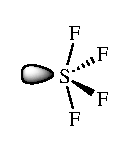
\includegraphics{picture/SF4.eps}
                \end{minipage}
            }
            \subfigure[\ce{SOF4}的结构]{
                \begin{minipage}[b]{.3\linewidth}
                    \centering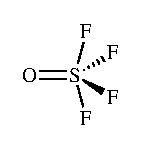
\includegraphics{picture/SOF4.eps}
                \end{minipage}
            }
            \subfigure[\ce{(H2C)SF4}的结构]{
                \begin{minipage}[b]{.3\linewidth}
                    \centering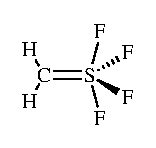
\includegraphics{picture/S(CH2)F4.eps}
                \end{minipage}
            }
            \caption{\ce{SF4}及其衍生物的结构}
        \end{figure}
        \ce{SF4}遇潮气迅速分解,并立即水解生成\ce{HF}和\ce{SO2}.尽管如此,在无机和有机合成中,它仍是具有高度选择性的强氟化剂,用途颇为广泛.
    \item \tbf{\ce{SF6}}\\
        \indent 六氟化硫\ce{SF6}可由硫在氟气氛中燃烧制得.它是无色,无臭,无味,无毒的气体\footnote{少量吸入\ce{SF6}可以让声音变得粗犷,这和吸入\ce{He}使得声音变细正好相反.请勿自行尝试此实验,以避免窒息风险.},无反应性和可燃性,也无溶解性.正由于它突出的稳定性和优良的绝缘性,广泛用作高压发电机和开关装置中的绝缘气体.\\
        \indent 近年来的最新观点认为\ce{SF6}中的\ce{S}并非VSEPR理论所认为的$\text{d}^2\text{sp}^3$杂化,而是采取sp杂化与两个\ce{F}成键,其余四个\ce{F}则与\ce{S}通过电性作用结合.经过平均化后,形成了正八面体的\ce{SF6}分子.
    \item \tbf{\ce{S2F10}}\\
        \indent 对硫的不完全氟化可以得到\ce{S2F10}分子.它的结构可以看作是两个\ce{SF6}各自去掉一个\ce{F}后两个\ce{S}相连的结果.由于没有特别的轨道作用,为了避免位阻,\ce{S2F10}采取交错式结构,其中的\ce{S-S}键也较长且弱.\\
        \indent \ce{S2F10}的反应性介于\ce{SF4}与\ce{SF6}之间.。它不为水所水解,甚至不为稀酸或稀碱所水解,这一点和\ce{SF4}不同;它作为剧毒物质也不同于\ce{SF6}.\ce{S2F10}在$15\tccentigrade$时迅速发生歧化,分解生成\ce{SF4}和\ce{SF6}.\\
        \indent \ce{S2F10}可以在丙酮溶液中氧化\ce{KI}而析出\ce{I2}.一个小把戏是还原产生的\ce{SF4}可以对丙酮进行氟化,因此反应的方程式应当为:
        \begin{center}
            \ce{S2F10 + 2KI + 4Me2CO -> 2SO2 + 2KF + I2 + 4Me2CF2}
        \end{center}
        下面是\ce{SF6}和\ce{S2F10}的结构.
        \begin{figure}[H]
            \centering
            \subfigure[\ce{SF6}的结构]{
                \begin{minipage}[b]{.45\linewidth}
                    \centering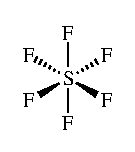
\includegraphics{picture/SF6.eps}
                \end{minipage}
            }
            \subfigure[\ce{S2F10}的结构]{
                \begin{minipage}[b]{.3\linewidth}
                    \centering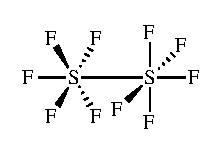
\includegraphics{picture/S2F10.eps}
                \end{minipage}
            }
            \caption{\ce{SF6}和\ce{S2F10}的结构}
        \end{figure}
\end{enumerate}
\subsubsection{硫的氯化物}
在剩余的硫的卤化物中,我们主要讨论最常见的\ce{SCl2}和\ce{S2Cl2},它们都是重要的化工产品.
\begin{substance}[\ce{SCl2}]
    二氯化硫,化学式为\ce{SCl2},是有毒且有恶臭味的樱桃红色液体,易挥发,熔点为$-122\tccentigrade$,沸点为$59\tccentigrade$.
\end{substance}
\begin{substance}[\ce{S2Cl2}]
    二氯化二硫,化学式为\ce{S2Cl2},是有毒且有恶臭味的金黄色液体,熔点为$-76\tccentigrade$,沸点为$138\tccentigrade$.
\end{substance}
\ce{S2Cl2}在热力学上比\ce{SCl2}更稳定.因此,如果某一反应应当生成硫的氯化物,在没有其它提示的情况下你可以优先考虑\ce{S2Cl2}的生成.\ce{SCl2}最著名的反应是对乙烯的硫代氯化:
\begin{center}
    \ce{SCl2 + C2H4 -> S(CH2CH2Cl)2}
\end{center}
产物即臭名昭著的芥子气.
\subsubsection{硫的氯氧化物}
硫可以形成两个主要系列的卤氧化物,即\ce{S^{IV}OX2}和\ce{S^{VI}O2X2}.我们主要介绍亚硫酰氯\ce{SOCl2}和硫酰氯\ce{SO2Cl2}.
\begin{substance}[\ce{SOCl2}]
    亚硫酰氯,化学式为\ce{SOCl2},是无色易挥发的液体,熔点为$-101\tccentigrade$,沸点为$76\tccentigrade$.
\end{substance}
\begin{substance}[\ce{SO2Cl2}]
    硫酰氯,化学式为\ce{SO2Cl2},也是无色易挥发的液体,熔点为$-54\tccentigrade$,沸点为$69\tccentigrade$.
\end{substance}
\ce{SOCl2}可以由\ce{SO2}氯化得到,亦可以由\ce{SCl2}被\ce{SO3}氧化得到:
\begin{center}
    \ce{SO2 + PCl5 -> SOCl2 + POCl3}\\
    \ce{SCl2 + SO3 -> SOCl2 + SO2}
\end{center}
\ce{SOCl2}能与\ce{H2O}剧烈作用,,可以对容易水解的无机卤化物进行脱水.以\ce{FeCl3.6H2O}为例:
\begin{center}
    \ce{FeCl3.6H2O + 6SOCl2 -> FeCl3 + 6SO2 + 6H2O}
\end{center}
与DMSO一样,\ce{SOCl2}也可以作为溶剂使用.\\
\indent 工业上用活性炭或\ce{FeCl3}为催化剂,将\ce{SO2}直接氯化就可以得到\ce{SO2Cl2}.这也是一种有用的氯化试剂.
\subsection{硫的氮化物}
\subsubsection{二元硫氮化合物}
这类物质中最重要的是\ce{S4N4}.这是一种橙黄色的晶体,在空气中稳定,但受到撞击或迅速加热时会发生爆炸.它可以通过下面几种方法制备:
\begin{center}
    \ce{6S2Cl2 + 16 NH3 ->T[$80\tccentigrade$] S4N4 + 8S + 12NH4Cl}\\
    \ce{6SCl2 + 16 NH3 -> S4N4 + 2S + 12NH4Cl}\\
    \ce{6S2Cl2 + 4NH4Cl ->T[$160\tccentigrade$] S4N4 + 8S + 16HCl}
\end{center}
\indent\ce{S4N4}具有耐人寻味的结构.
\begin{figure}[H]
    \centering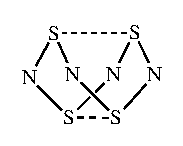
\includegraphics{picture/S4N4.eps}
    \caption{\ce{S4N4}的立体结构}
\end{figure}
\ce{S4N4}分子隶属$D_{2\text d}$点群,\ce{S-N}键长小于单键键长,表明杂环中有一定的离域效应.跨环的\ce{S-S}有一定的成键作用.\\
\indent \ce{S4N4}在碱中水解,水解产物与碱的浓度有关:
\begin{center}
    \ce{2S4N4 + 6OH- + 9H2O ->T[稀碱] S2O3^2- + 2S3O6^2- + 8NH3}\\
    \ce{S4N4 + 6OH- + 3H2O ->T[浓碱] S2O3^2- + 2SO3^2- + 4NH3}
\end{center}
\subsection{硫的多原子阳离子}
为了保持连续性,这部分内容将和\ce{Se},\ce{Te}的多原子阳离子一起介绍.
\end{document}